\documentclass[aspectratio=169,11pt]{beamer}
\usepackage{beamerucad}
\usepackage{listings}
\definecolor{ckw}{HTML}{2563AB}\definecolor{cst}{HTML}{2E8B57}\definecolor{ccm}{HTML}{8A8F98}
\lstdefinestyle{jv}{language=Java,basicstyle=\ttfamily\footnotesize,
 keywordstyle=\color{ckw}\bfseries,stringstyle=\color{cst},commentstyle=\color{ccm}\itshape,
 showstringspaces=false,columns=fullflexible,keepspaces=true,
 backgroundcolor=\color{ucadband!8},frame=leftline,framerule=2.5pt,rulecolor=\color{ucadband},
 xleftmargin=8pt,aboveskip=3pt,belowskip=1pt,basewidth=0.5em}
\lstset{style=jv}
\title{Architectures Logicielles — Séance 1}
\subtitle{Du chaos aux couches : juger, diagnostiquer et refactorer une structure}
\author{Dr. El Hadji Bassirou TOURÉ}
\institute{Département de Mathématiques et Informatique\\ Faculté des Sciences et Techniques\\ Université Cheikh Anta Diop de Dakar}
\date{}
\setucadfoot{Architectures Logicielles --- Séance 1 \quad\textbullet\quad Dr. El Hadji Bassirou TOURÉ --- DMI/FST/UCAD}
\graphicspath{{figs/}}
\begin{document}

\begin{frame}[plain,noframenumbering]\titlepage\end{frame}

\begin{frame}{Objectifs de la séance}
\begin{ucaddef}[Contenu]
{\small Cette séance pose le socle du cours : ce qu'est une \textbf{architecture logicielle}, comment on la \textbf{juge} (attributs de qualité), comment on la \textbf{diagnostique} (couplage, cohésion), et comment on l'\textbf{améliore en sécurité} (refactoring vers une architecture en couches). Le lab applique tout cela à SénResto, notre plateforme de livraison de repas à Dakar.}
\end{ucaddef}
\begin{itemize}\small
  \item Distinguer \emph{fonctionner} et \emph{être bien structuré} : la notion de \textbf{dette architecturale}.
  \item Juger une structure avec les \textbf{attributs de qualité} — et comprendre qu'ils se paient les uns avec les autres.
  \item Diagnostiquer avec le vocabulaire du métier : \textbf{couplage} et \textbf{cohésion}.
  \item Connaître le remède du jour, l'\textbf{architecture en couches}, et la méthode sûre pour y aller : le \textbf{refactoring} protégé par des tests.
\end{itemize}
\end{frame}

% #####################################################################
\section{Fonctionner ne suffit pas}

\begin{frame}{Le patient du jour : SénResto}
\begin{ucaddef}[La situation]
{\small SénResto permet de commander un thiéboudienne chez Fatou à la Médina ou un mafé chez Aminata à Ouakam, d'assigner un livreur et de suivre la commande jusqu'à la livraison. L'application \textbf{fonctionne parfaitement} : le frontend React est agréable, l'API répond, les livreurs sont assignés, les montants sont justes.}
\end{ucaddef}
\vskip2pt
{\small Et pourtant : tout le backend tient dans \textbf{une seule classe de 414 lignes}. La question de la séance --- et du semestre :}
\begin{ucadpiege}[La question centrale]
{\small Si l'application fonctionne, qu'est-ce qui ne va pas ? \emph{Pour qui} est-elle mauvaise, et \emph{quand} cela se paiera-t-il ?}
\end{ucadpiege}
\end{frame}

\begin{frame}{Qu'est-ce qu'une architecture logicielle ?}
\begin{ucaddef}[Définition]
{\small L'\textbf{architecture} d'un logiciel est sa structure : les \textbf{parties} qui le composent, la \textbf{responsabilité} de chacune, et les \textbf{dépendances} entre elles. Ce sont les décisions structurantes — celles qui seraient \emph{coûteuses à changer} une fois prises.}
\end{ucaddef}
\begin{itemize}\small
  \item Ajouter un bouton se défait en une heure : ce n'est pas de l'architecture.
  \item Décider que tout le code vit dans une classe — ou dans trois couches, ou dans cinq services — engage \emph{tout} le développement futur : c'est de l'architecture.
\end{itemize}
\begin{ucadret}[À retenir]
{\small L'architecture ne se voit pas à l'écran. Deux applications identiques pour l'utilisateur peuvent être, pour l'équipe qui les maintient, un plaisir ou un cauchemar.}
\end{ucadret}
\end{frame}

\begin{frame}{L'intuition du restaurant}
\begin{ucadex}[Un restaurant bien organisé]
{\small En salle, le serveur prend les commandes et sert — il ne cuisine pas. En cuisine, le chef applique les recettes — il ne fait pas le service. Au cellier, le magasinier gère les stocks — il ne cuisine pas. Chacun a \textbf{un métier}, et la commande circule dans \textbf{un seul sens} : salle $\to$ cuisine $\to$ cellier.}
\end{ucadex}
\vskip2pt
{\small Imaginez maintenant le restaurant où \emph{une seule personne} prend les commandes, cuisine, gère le stock et encaisse. Ça marche... tant qu'il y a trois clients, et tant qu'elle ne tombe pas malade. C'est exactement l'état de SénResto aujourd'hui.}
\begin{ucadret}[À retenir]
{\small Une bonne structure permet de comprendre, modifier, tester et remplacer chaque partie \textbf{séparément}. C'est vrai d'un restaurant, c'est vrai d'un logiciel.}
\end{ucadret}
\end{frame}

% #####################################################################
\section{Attributs de qualité}

\begin{frame}{La dette architecturale}
\begin{ucaddef}[Dette architecturale]
{\small La \textbf{dette architecturale} est le coût futur créé par les raccourcis structurels d'aujourd'hui. Comme une dette d'argent, elle porte intérêt : chaque fonctionnalité coûte plus cher que la précédente.}
\end{ucaddef}
\centering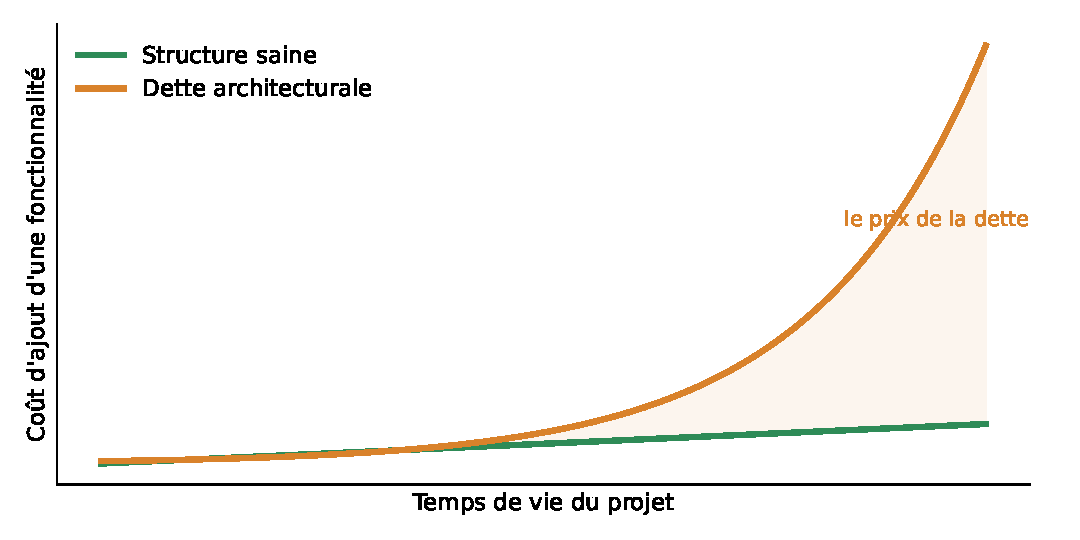
\includegraphics[width=0.50\linewidth]{figA_cout_changement}

{\scriptsize Au début, les deux courbes se confondent — la mauvaise structure est même souvent \emph{plus rapide}. C'est pour cela qu'on la choisit... et qu'on la regrette.}
\end{frame}

\begin{frame}{Les attributs de qualité}
\begin{ucaddef}[Attributs de qualité]
{\small Les \textbf{attributs de qualité} sont les propriétés non fonctionnelles par lesquelles on juge une structure. Chacun se traduit par une question concrète et vérifiable.}
\end{ucaddef}
\vskip2pt
{\small\begin{tabular}{p{0.24\linewidth}p{0.66\linewidth}}
\toprule
\textbf{Attribut} & \textbf{La question concrète}\\
\midrule
Maintenabilité & Combien de fichiers faut-il toucher pour ajouter un quartier livrable ?\\
Testabilité & Peut-on vérifier la formule des frais \emph{sans} démarrer une base de données ?\\
Évolutivité & Ajouter le paiement mobile money : chantier local ou refonte générale ?\\
Lisibilité & Un nouveau membre du groupe comprend-il où vit chaque règle ?\\
Résilience & Si une partie tombe, le reste survit-il ? (rendez-vous au Lab 5)\\
\bottomrule
\end{tabular}}
\end{frame}

\begin{frame}{Les trade-offs}
\begin{ucaddef}[Trade-off]
{\small Un \textbf{trade-off} est un échange : améliorer un attribut se paie presque toujours en dégradant un autre. Il n'existe pas de « meilleure architecture » dans l'absolu — seulement des architectures \emph{adaptées à un contexte}.}
\end{ucaddef}
\begin{itemize}\small
  \item Séparer en couches améliore la testabilité... au prix de \emph{plus de fichiers} et d'indirection.
  \item Les microservices améliorent le déploiement indépendant... au prix de la complexité du réseau (nous le \emph{vivrons} au Lab 4).
\end{itemize}
\begin{ucadret}[À retenir — la devise du semestre]
{\small Un architecte ne demande jamais « quelle est la meilleure solution ? » mais « \textbf{qu'est-ce que j'achète, et avec quoi je le paie ?} ». Chaque ADR que vous rédigerez devra nommer ce qui est payé.}
\end{ucadret}
\end{frame}

% #####################################################################
\section{Couplage et cohésion}

\begin{frame}{Le couplage}
\begin{ucaddef}[Définition]
{\small Le \textbf{couplage} mesure à quel point les parties d'un système dépendent les unes des autres. Il se lit dans une question : \emph{si je modifie ceci, qu'est-ce que je risque de casser ?}}
\end{ucaddef}
\centering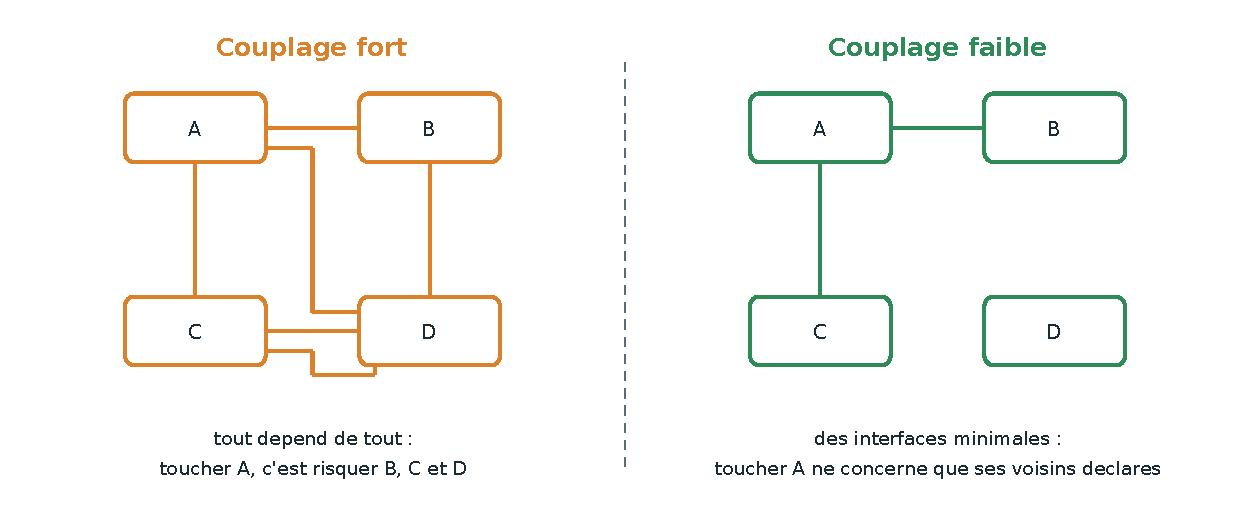
\includegraphics[width=0.72\linewidth]{figB_couplage}
\end{frame}

\begin{frame}{La cohésion}
\begin{ucaddef}[Définition]
{\small La \textbf{cohésion} mesure à quel point les éléments regroupés ensemble le sont \emph{pour une bonne raison} — parce qu'ils participent à la même responsabilité.}
\end{ucaddef}
\begin{ucadex}[Test rapide sur SénResto]
{\small Décrivez \texttt{SenRestoController} en une phrase sans dire « et » : \emph{« il reçoit les requêtes HTTP \textbf{et} valide les données \textbf{et} calcule les frais \textbf{et} écrit le SQL \textbf{et} assigne les livreurs \textbf{et} envoie les SMS... »} Chaque « et » est un aveu : la classe a plusieurs métiers, sa cohésion est faible.}
\end{ucadex}
\begin{ucadret}[La devise]
{\small \textbf{Couplage faible, cohésion forte.} Chaque module fait une chose (cohésion), et dépend du minimum d'autres modules (couplage). C'est le principe de responsabilité unique, à toutes les échelles.}
\end{ucadret}
\end{frame}

\begin{frame}{Les symptômes au microscope : SénResto}
\centering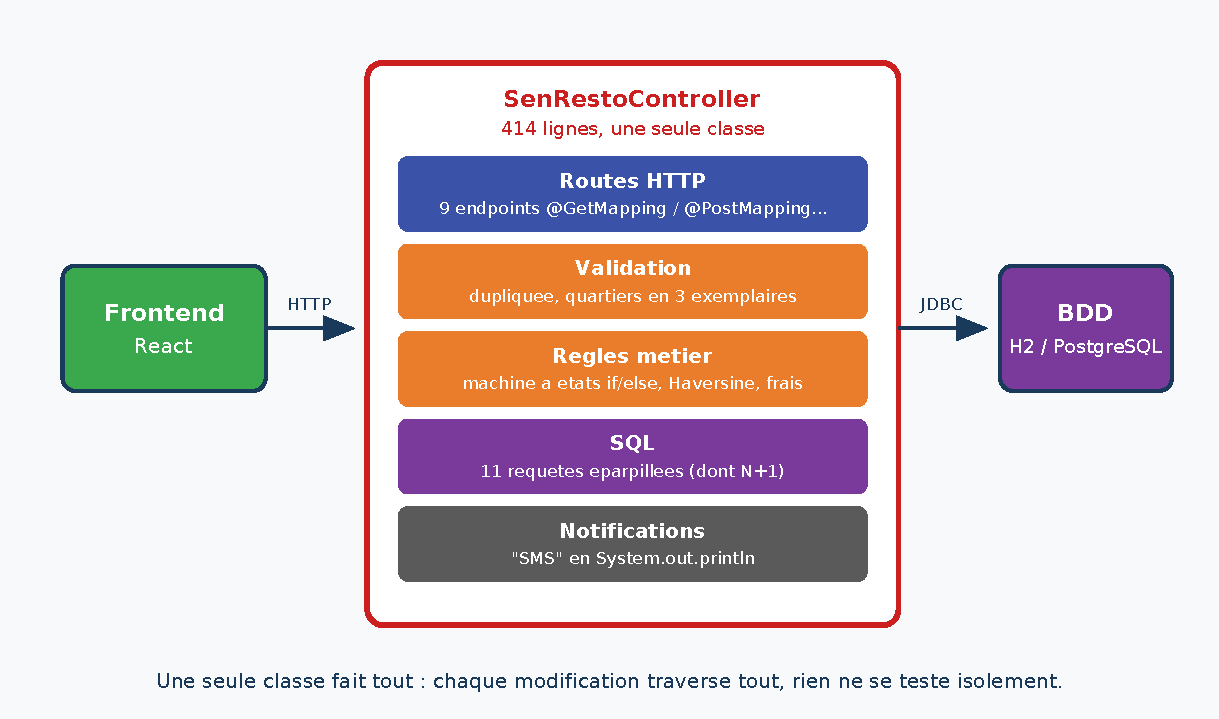
\includegraphics[width=0.70\linewidth]{fig1_god_controller}

{\scriptsize Un \emph{God controller} : toutes les responsabilités dans une classe. Au lab, vous cartographierez ligne par ligne les sept défauts de cette structure.}
\end{frame}

\begin{frame}{Le symptôme qui les résume tous}
\begin{ucadpiege}[Rien ne se teste isolément]
{\small Pour vérifier la simple formule « prix $\times$ quantité $+$ frais », il faut aujourd'hui : démarrer Spring, initialiser une base de données, construire une requête HTTP, et analyser du JSON. La règle métier est \textbf{prisonnière} de la technique qui l'entoure.}
\end{ucadpiege}
\begin{itemize}\small
  \item C'est pour cela que le projet ne contient \emph{que} des tests d'intégration : le test unitaire y est \textbf{impossible} — non pas difficile, impossible.
  \item La testabilité est le \textbf{thermomètre} de l'architecture : un code difficile à tester est un code mal structuré. L'inverse est (presque) toujours vrai.
\end{itemize}
\begin{ucadex}[Vérité de terrain]
{\small La duplication aggrave tout : la liste des quartiers de Dakar existe en \textbf{trois} exemplaires (frais, GPS, formulaire React). Ouvrir la livraison aux Parcelles Assainies = trois modifications à ne pas oublier. La probabilité d'oubli croît avec le temps... et se découvre en production.}
\end{ucadex}
\end{frame}

% #####################################################################
\section{L'architecture en couches}

\begin{frame}{Trois couches, trois métiers}
\centering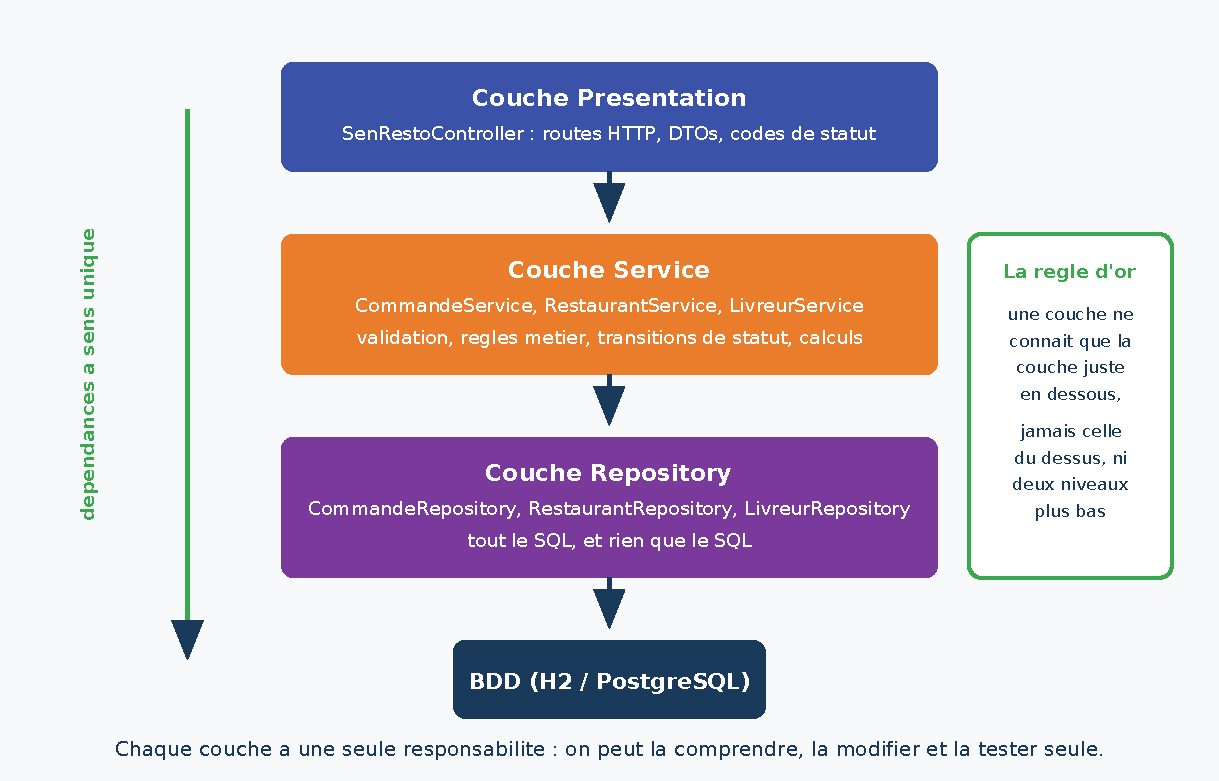
\includegraphics[width=0.60\linewidth]{fig2_couches}
\end{frame}

\begin{frame}{La responsabilité de chaque couche}
{\small\begin{tabular}{p{0.22\linewidth}p{0.36\linewidth}p{0.32\linewidth}}
\toprule
\textbf{Couche} & \textbf{Son métier} & \textbf{Ce qu'elle s'interdit}\\
\midrule
Présentation \newline (\texttt{controller}) & parler HTTP : routes, codes de statut, sérialisation & toute règle métier, tout SQL\\
\addlinespace
Service \newline (\texttt{service}) & le métier : validation, règles, calculs, transitions d'état & parler HTTP, parler SQL\\
\addlinespace
Accès aux données \newline (\texttt{repository}) & tout le SQL, et rien que le SQL & valider, décider, calculer\\
\bottomrule
\end{tabular}}
\vskip4pt
\begin{ucadret}[La règle d'or]
{\small Les dépendances vont dans \textbf{un seul sens}, du haut vers le bas, et chaque couche ne connaît que sa voisine immédiate. Le controller ignore la base ; le repository ignore HTTP.}
\end{ucadret}
\end{frame}

\begin{frame}[fragile]{Ce que la séparation achète}
{\small Avant : la validation vit \emph{dans} l'endpoint, testable uniquement via HTTP + BDD. Après : elle vit dans le service, et lève une exception métier — testable en une ligne, sans rien démarrer :}
\begin{lstlisting}
// Dans CommandeService : du metier pur, sans HTTP ni SQL
private String validerTelephone(Object tel) {
    if (tel == null || !tel.toString().matches("^7[05678][0-9]{7}$")) {
        throw new ValidationException("Telephone invalide : format 7XXXXXXXX");
    }
    return tel.toString();
}
\end{lstlisting}
\begin{itemize}\small
  \item Un seul \texttt{@RestControllerAdvice} traduit les exceptions métier en codes HTTP — là où le God controller répétait neuf fois le même bloc d'erreur.
  \item La règle des frais, la machine à états, le calcul d'ETA deviennent des méthodes \textbf{nommées}, à \textbf{une} adresse, testables \textbf{unitairement}.
\end{itemize}
\end{frame}

% #####################################################################
\section{Refactorer en sécurité}

\begin{frame}{Le refactoring : définition et contrat}
\begin{ucaddef}[Définition]
{\small Le \textbf{refactoring} consiste à améliorer la structure interne d'un code \textbf{sans changer son comportement observable}. Mêmes routes, mêmes JSON, mêmes codes d'erreur : le frontend ne doit rien remarquer du chantier.}
\end{ucaddef}
\begin{ucadpiege}[Le piège classique]
{\small « Tant qu'on y est, corrigeons aussi ce petit bug... » — Non. Changer le comportement \emph{pendant} un refactoring, c'est perdre son juge de paix : un test casse, et on ne sait plus si c'est la structure ou le comportement. \textbf{Une intention à la fois.}}
\end{ucadpiege}
\begin{ucadrec}[La méthode des petits pas]
{\small Extraire \emph{une} responsabilité $\to$ relancer les tests $\to$ committer $\to$ recommencer. Le refactoring avance en pas de fourmi, mais il n'échoue jamais.}
\end{ucadrec}
\end{frame}

\begin{frame}[fragile]{Le filet : les tests de comportement}
{\small Le projet fournit \textbf{quatre tests d'intégration} qui décrivent le comportement de l'API — et ignorent tout de sa structure interne. C'est précisément pour cela qu'ils survivront au refactoring :}
\begin{lstlisting}
./mvnw test
# Tests run: 4, Failures: 0, Errors: 0   <- l'etat obligatoire, en permanence
\end{lstlisting}
\begin{itemize}\small
  \item Lister les restaurants, créer une commande, rejeter un téléphone invalide, confirmer et assigner un livreur : les quatre parcours vitaux.
  \item \textbf{Un test rouge = le comportement a changé = ce n'est plus du refactoring.} On revient en arrière (\texttt{git}), on comprend, on recommence plus petit.
\end{itemize}
\begin{ucadret}[À retenir]
{\small On ne refactore jamais sans filet. Les tests transforment une opération à c\oe ur ouvert en une promenade balisée.}
\end{ucadret}
\end{frame}

\begin{frame}{Le chemin du lab, tag par tag}
\centering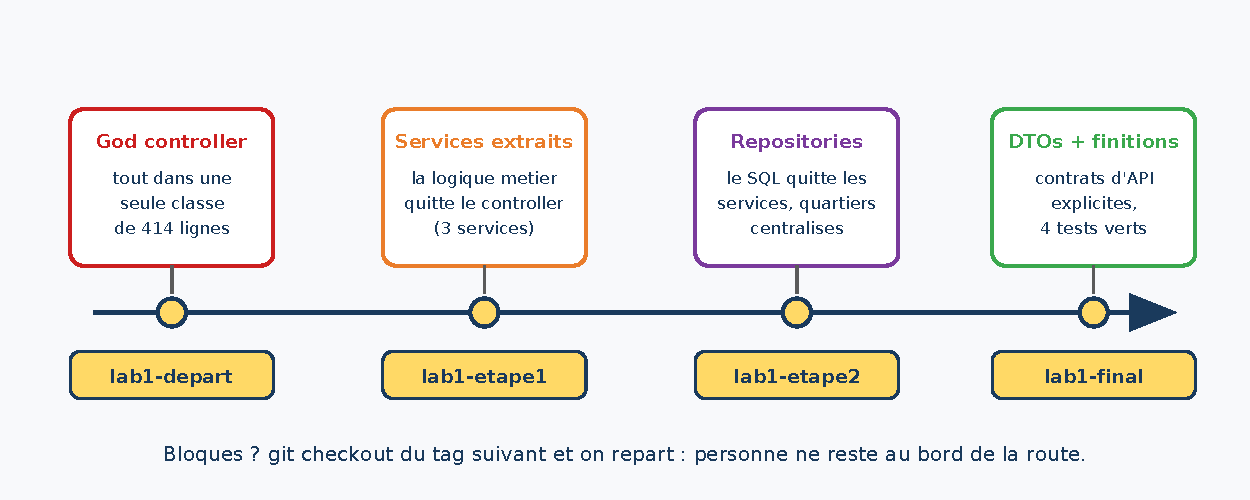
\includegraphics[width=0.80\linewidth]{fig3_chemin_tags}

{\scriptsize Le code de départ de chaque lab du semestre sera l'état final du lab précédent : rester dans le rythme, c'est capitaliser.}
\end{frame}

\begin{frame}{Votre mission d'aujourd'hui}
{\scriptsize\begin{tabular}{p{0.20\linewidth}p{0.72\linewidth}}
\toprule
\textbf{Rôle} & \textbf{Pilotage au Lab 1}\\
\midrule
Le Doyen & branches \texttt{feature/}, merges, tags — et l'ADR avec l'Architecte du jour\\
L'Huissier & \texttt{CommandeService}, exceptions métier, \texttt{GestionnaireErreurs}\\
Le Rédacteur & \texttt{RestaurantService}, puis les DTOs (le contrat de \emph{son} frontend)\\
Le Notaire & l'inventaire SQL, puis les trois repositories\\
L'Appariteur & \texttt{LivreurService}, \texttt{QuartiersDakar}, vérification H2 + PostgreSQL\\
\bottomrule
\end{tabular}}
\vskip4pt
\begin{ucadrec}[Le livrable individuel de la séance]
{\small L'\textbf{Architecte du jour} signe l'\textbf{ADR n\textsuperscript{o}1 : « Pourquoi séparer en couches ? »} — une page, deux alternatives sérieuses, deux conséquences négatives assumées (gabarit distribué).}
\end{ucadrec}
\end{frame}

\begin{frame}{L'essentiel de la séance}
\begin{ucadret}[À retenir]
{\footnotesize
\begin{itemize}
  \item \textbf{Fonctionner ne suffit pas} : la dette architecturale se contracte en silence et se paie avec intérêts.
  \item On juge une structure par ses \textbf{attributs de qualité}, et on sait qu'ils s'achètent les uns avec les autres : \textbf{trade-offs}.
  \item Le diagnostic tient en une devise : \textbf{couplage faible, cohésion forte} — et la testabilité en est le thermomètre.
  \item Le remède du jour : \textbf{trois couches}, des dépendances à sens unique — atteintes par \textbf{petits pas}, sous la protection des tests, jalonnées par les tags.
\end{itemize}}
\end{ucadret}
\begin{ucadfront}[La question qui ouvre la séance 2]
{\footnotesize Votre code sera propre ce soir... mais vos règles métier dépendront toujours, trois étages plus bas, d'une base de données. Peut-on \emph{retourner} cette dépendance comme un gant ? Réponse au Lab 2 : l'architecture hexagonale.}
\end{ucadfront}
\end{frame}

\end{document}
